%Appendix: detailed information on collaboration and links to the main sources

\appendix
\beginbackup
\section{Appendix}
\subsection{Collaboration}
\begin{frame}[allowframebreaks]
{The German-Russian Astroparticle Data Life Cycle collaboration}
\parbox{0.35\textwidth}{
  \centering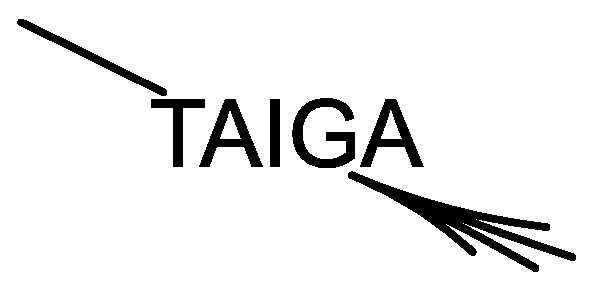
\includegraphics[width=0.25\textwidth]{pics/taiga.eps}
}\hfill
\parbox{0.60\textwidth}{
  TAIGA---Tunka Advanced Instrument for cosmic ray physics and Gamma Astronomy (see
%       https://
  taiga-experiment.info);
}
\\\vspace{1em}
\parbox{0.35\textwidth}{
  \centering
\includegraphics[width=0.35\textwidth]{pics/grande.pdf}
}\hfill
\parbox{0.60\textwidth}{
  KASCADE-Grande---KArlsruhe Shower Core and Array DEtector---Grande\\ (see
%       http://
  www-ik.fzk.de/KASCADE\_home.html);
}
\\\vspace{1em}
\parbox{0.35\textwidth}{
  \centering
\includegraphics[width=0.30\textwidth]{pics/Logo_KIT_IKP.pdf}
}\hfill
\parbox{0.60\textwidth}{
  KIT-IKP---Institute for Nuclear Physics Karlsruhe Institute of Technology
}
\\\vspace{1em}
\parbox{0.35\textwidth}{
  \centering
\includegraphics[width=0.15\textwidth]{pics/SCC-Logo.png}
}\hfill
\parbox{0.60\textwidth}{
  SCC---Steinbuch Centre for Computing Karlsruhe Institute of Technology
}
\\\vspace{1em}
\parbox{0.20\textwidth}{
  \centering
\includegraphics[width=0.20\textwidth]{pics/SINP_MSU_LOGO.pdf}
}\hfill
\parbox{0.75\textwidth}{
  SINP MSU---Skobeltsyn Institute Of Nuclear Physics Lomonosov Moscow State University
}
\\\vspace{1em}
\parbox{0.20\textwidth}{
  \centering
\includegraphics[width=0.15\textwidth]{pics/isu_logo.png}
}\hfill
\parbox{0.75\textwidth}{
  ISU---Irkutsk State University
}
\\\vspace{1em}
\parbox{0.20\textwidth}{
  \centering
\includegraphics[width=0.18\textwidth]{pics/matr_logo.png}
}\hfill
\parbox{0.75\textwidth}{
  ISDCT---Matrosov Institute for System Dynamics and Control Theory
}
\end{frame}

\subsection{References}
    \begin{frame}{References}
        \begin{itemize}
            \item Berghöfer T., Agrafioti I. \textit{et al.} Towards a model for computing in European astroparticle physics,
            Astroparticle Physics European Coordination committee, 2016,
            web-source:~\texttt{http://appec.org/wp-content/uploads/\\Documents/Docs-from-old-site/AModelForComputing-2.pdf};
            \item KCDC---\textbf{K}ASCADE \textbf{C}osmic Ray \textbf{D}ata \textbf{C}enter,\\
            web-source:~\texttt{http://kcdc.ikp.kit.edu};
            \item KASCADE-Grande official site, web-source:~\texttt{http://www-ik.fzk.de/KASCADE\_home.html};
            \item TAIGA collaboration official site, web-source:~\texttt{http://taiga-experiment.info};
            \item Astroparticle.online---outreach resource, web-source:~\texttt{http://astroparticle.online}.
        \end{itemize}
    \end{frame}
\backupend